\documentclass[11pt,letterpaper]{article}

\usepackage[spanish,es-noshorthands]{babel}
\usepackage{fontspec}
\setmainfont{Source Serif Pro}
\usepackage{microtype}
\usepackage{geometry}
\usepackage{booktabs}
\usepackage{tabularx}
\usepackage{enumitem}
\usepackage{xcolor}
\usepackage{graphicx}
\usepackage{csquotes}
\usepackage{amsmath}
\usepackage{siunitx}
\usepackage{tikz}
\usetikzlibrary{arrows.meta,positioning,shapes.geometric,fit,backgrounds}
\usepackage{xurl}
\usepackage[hidelinks]{hyperref}
\usepackage[backend=biber,style=apa,sorting=nyt]{biblatex}
\DeclareLanguageMapping{spanish}{spanish-apa}

\geometry{margin=2.3cm}
\setlength{\emergencystretch}{1em}
\setlength{\parindent}{0pt}
\setlength{\parskip}{0.55em}
\setlist{nosep}
\addbibresource{referencias.bib}
\AtBeginBibliography{\sloppy}

\sisetup{
  output-decimal-marker = {,},
  group-separator = {.},
  group-minimum-digits = 4,
  detect-all
}

\title{\vspace{-1.2cm}\textbf{Modelo conceptual en OPM de la patente 528.671}\\
\large De una descripción de piezas numeradas a un modelo de función:
la trampa para ratones}
\author{Carlos Luis Rojas Aragonés\\
\small Gestión del Desarrollo Tecnológico}
\date{\small 8 de agosto de 2026}

\begin{document}

\maketitle
\vspace{-0.8em}

\section*{Qué se modela y con qué criterio}

El fragmento de la patente 528.671, concedida en Estados Unidos en 1894 a
William C. Hooker \parencite{hooker1894}, describe una trampa para ratones
enumerando catorce piezas y explicando cómo se doblan, se perforan y se sujetan
entre sí. Es un texto de \emph{forma}: dice de qué está hecho el artefacto y
cómo se ensambla, pero en ningún momento enuncia qué hace ni en qué orden. La
metodología objeto-proceso (OPM) sirve exactamente para recuperar lo segundo,
porque obliga a colocar en el mismo diagrama las dos clases de entidad que el
lenguaje natural mezcla: los objetos, que existen, y los procesos, que
transforman objetos \parencite{dori2002,iso19450}.

El procedimiento de traducción que seguí es el habitual y es casi mecánico.
Los sustantivos que persisten se convierten en \textbf{objetos} (base, gatillo,
martillo, muelle transversal); los adjetivos y las condiciones en que puede
estar cada uno se convierten en \textbf{estados} (armada, tensionado,
enganchado); los verbos que producen un cambio de estado se convierten en
\textbf{procesos} (armar, liberar, descargar, golpear, sujetar). El criterio de
corte fue funcional: una pieza de la patente entra al modelo como objeto propio
solo si alguno de sus estados cambia durante la operación. Por eso los vástagos
(7), las perforaciones (6), el pivote (13) o el perno (14) no aparecen como
objetos: son detalles de ensamblaje que no cambian de estado y que la propia
patente admite variar, hasta el punto de decir que el gatillo puede fabricarse
\enquote{con cualquier material compatible}. Esa asimetría entre una forma
sustituible y una función invariante es la razón de ser del modelo
\parencite{crawley2016}.

\section*{El diagrama de objeto-proceso}

La Figura~\ref{fig:opd} reproduce el diagrama construido en OPM Sandbox. La
notación se lee así: los rectángulos verdes son objetos, las elipses azules son
procesos, los rectángulos redondeados dentro de un objeto son sus estados, el
triángulo negro es una relación de agregación y las líneas terminadas en círculo
conectan procesos con los objetos que consumen, usan o transforman.

\begin{figure}[ht]
  \centering
  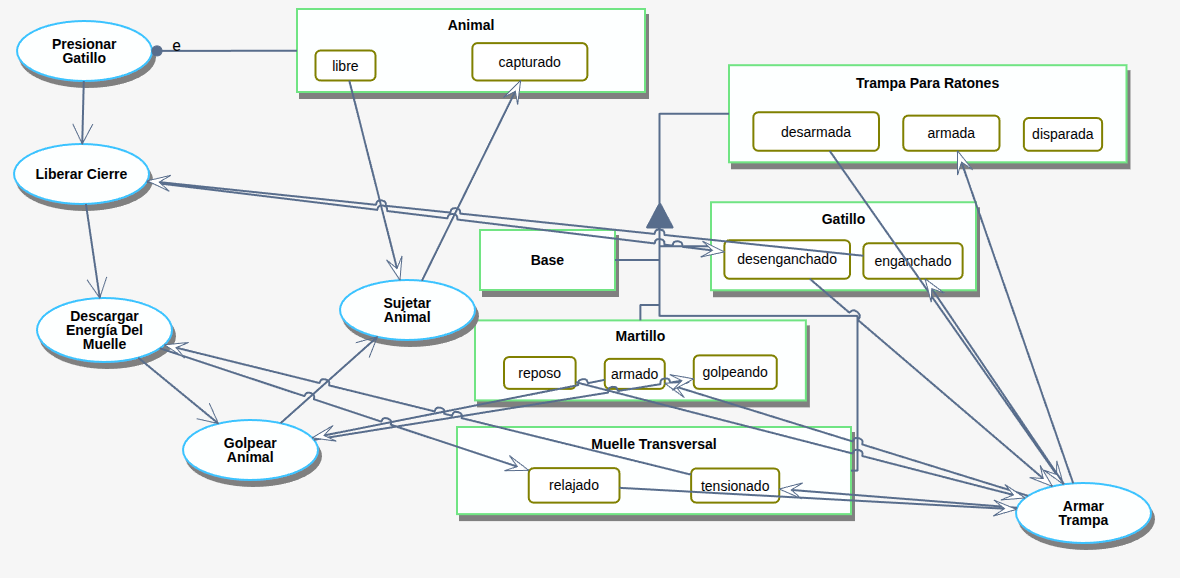
\includegraphics[width=\textwidth]{OPM Mouse Trap.png}
  \caption{Diagrama de objeto-proceso (OPD) de la trampa para ratones de la
  patente 528.671, elaborado en OPM Sandbox. Un único diagrama contiene la
  estructura (la trampa se compone de base, gatillo, martillo y muelle
  transversal), el espacio de estados de cada objeto y los seis procesos que lo
  recorren.}
  \label{fig:opd}
\end{figure}

El modelo tiene seis objetos. \textbf{Trampa Para Ratones} es el todo, con tres
estados que describen su situación global: \emph{desarmada}, \emph{armada} y
\emph{disparada}. De él cuelgan por agregación cuatro partes: \textbf{Base},
que no tiene estados porque su papel es puramente estructural y no cambia nunca;
\textbf{Muelle Transversal}, que alterna entre \emph{relajado} y
\emph{tensionado}; \textbf{Martillo}, con tres estados (\emph{reposo},
\emph{armado} y \emph{golpeando}); y \textbf{Gatillo}, que está
\emph{enganchado} o \emph{desenganchado}. Fuera de la agregación queda
\textbf{Animal}, que puede estar \emph{libre} o \emph{capturado} y que además es
el agente que inicia la secuencia: el círculo negro que une Animal con Presionar
Gatillo es un enlace de agente, es decir, la entidad que decide y ejecuta el
proceso sin ser transformada por él.

Los procesos son seis y se reparten en dos episodios distintos. El primero es
\textbf{Armar Trampa}, que es el único momento en que interviene la persona que
coloca la trampa y el único proceso que modifica cuatro objetos a la vez: pasa
la trampa de desarmada a armada, el martillo de reposo a armado, el muelle de
relajado a tensionado y el gatillo de desenganchado a enganchado. El segundo
episodio es la cadena de disparo, que la patente describe en desorden a lo largo
de tres párrafos y que el diagrama ordena en cinco pasos encadenados: Presionar
Gatillo, Liberar Cierre, Descargar Energía Del Muelle, Golpear Animal y Sujetar
Animal.

\section*{El OPL: el mismo modelo dicho en frases}

La propiedad más útil de OPM para un informe de patente es que el modelo es
bimodal: el diagrama y un texto en lenguaje casi natural son dos vistas del
mismo modelo, generadas a la vez, de modo que ninguna puede desmentir a la otra
\parencite{dori2016}. La Figura~\ref{fig:opl} muestra el \emph{Object-Process
Language} que la herramienta produjo automáticamente a partir del diagrama. Las
palabras de estructura vienen en inglés (\emph{can be}, \emph{consists of},
\emph{changes \dots{} from \dots{} to}) porque las genera el motor de la
herramienta, mientras que los nombres de objetos, estados y procesos están en
español porque son los que yo introduje.

\begin{figure}[ht]
  \centering
  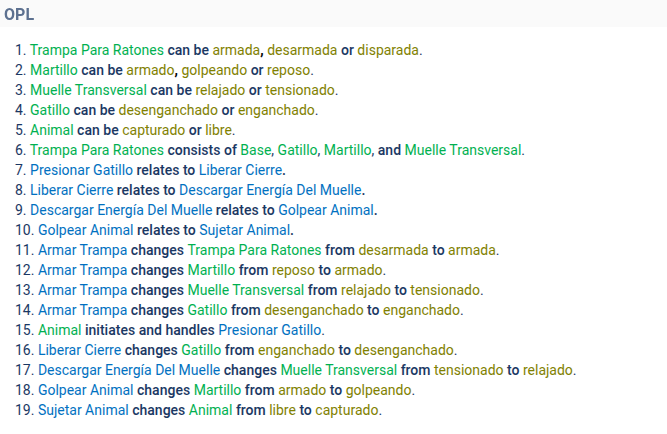
\includegraphics[width=0.86\textwidth]{OPL Mouse Trap.png}
  \caption{Object-Process Language (OPL) generado automáticamente a partir del
  diagrama de la Figura~\ref{fig:opd}. Las diecinueve frases son el modelo
  completo: cinco declaran espacios de estados, una declara la composición del
  artefacto, cuatro ordenan la secuencia de procesos y nueve describen los
  cambios de estado que cada proceso produce.}
  \label{fig:opl}
\end{figure}

Las diecinueve frases se agrupan en cuatro bloques que conviene leer por
separado. Las frases 1 a 5 declaran el espacio de estados de cada objeto y son,
en la práctica, el inventario de todo lo que la trampa puede llegar a ser. La
frase 6 declara la estructura: la trampa consiste en base, gatillo, martillo y
muelle transversal. Las frases 7 a 10 encadenan los procesos en el orden causal
del disparo. Y las frases 11 a 19 son el corazón del modelo, porque cada una
nombra un proceso, el objeto que altera y la transición concreta de estado que
produce: \enquote{Armar Trampa cambia Muelle Transversal de relajado a
tensionado}, \enquote{Liberar Cierre cambia Gatillo de enganchado a
desenganchado}, y así hasta \enquote{Sujetar Animal cambia Animal de libre a
capturado}. Una frase suelta, la 15, no describe una transformación sino una
responsabilidad: el animal inicia y ejecuta el acto de presionar el gatillo.

\section*{La cadena funcional y su correspondencia con el texto}

La Figura~\ref{fig:cadena} resume la lógica que el modelo extrae del texto: un
proceso previo carga el sistema con energía y establece cuatro precondiciones
simultáneas; después, una perturbación mínima libera esa energía en cascada.

\begin{figure}[ht]
  \centering
  \begin{tikzpicture}[
    proc/.style={draw, rounded corners=3mm, align=center, font=\small,
      text width=2.62cm, minimum height=10mm, fill=blue!7},
    nota/.style={align=center, font=\scriptsize, text width=2.8cm,
      color=black!65},
    fl/.style={-{Stealth[length=2mm]}, thick}
  ]
    \node[proc, fill=orange!14, text width=3.4cm] (armar) at (0,1.75)
      {\textbf{Armar Trampa}};
    \node[nota, text width=5.2cm, right=3mm of armar]
      {establece cuatro precondiciones a la vez: trampa \emph{armada}, muelle
       \emph{tensionado}, martillo \emph{armado}, gatillo \emph{enganchado}};

    \node[proc] (p1) at (0,0)     {Presionar\\Gatillo};
    \node[proc] (p2) at (3.15,0)  {Liberar\\Cierre};
    \node[proc] (p3) at (6.3,0)   {Descargar\\Energía};
    \node[proc] (p4) at (9.45,0)  {Golpear\\Animal};
    \node[proc] (p5) at (12.6,0)  {Sujetar\\Animal};

    \foreach \a/\b in {p1/p2, p2/p3, p3/p4, p4/p5} {
      \draw[fl] (\a) -- (\b);
    }
    \draw[fl, dashed, orange!60!black] (armar.south) -- (p1.north);

    \node[nota, below=2.5mm of p1] {agente: \emph{Animal}\\energía mínima};
    \node[nota, below=2.5mm of p2] {Gatillo:\\enganchado
      $\rightarrow$ desenganchado};
    \node[nota, below=2.5mm of p3] {Muelle:\\tensionado
      $\rightarrow$ relajado};
    \node[nota, below=2.5mm of p4] {Martillo:\\armado
      $\rightarrow$ golpeando};
    \node[nota, below=2.5mm of p5] {Animal:\\libre $\rightarrow$ capturado};
  \end{tikzpicture}
  \caption{Los dos episodios del modelo. Arriba, el único proceso que
  interviene una persona y que carga el sistema. Abajo, la cadena de disparo con
  la transición de estado que aporta cada paso. Elaboración propia a partir del
  modelo de las figuras \ref{fig:opd} y \ref{fig:opl}.}
  \label{fig:cadena}
\end{figure}

El Cuadro~\ref{tab:trazabilidad} cierra el círculo con el texto original: para
cada pieza numerada de la patente indica en qué entidad del modelo quedó
representada, o por qué no aparece.

\begin{table}[ht]
  \centering
  \small
  \caption{Trazabilidad entre las piezas numeradas de la patente y las entidades
  del modelo OPM.}
  \label{tab:trazabilidad}
  \begin{tabularx}{\textwidth}{@{}c
    >{\raggedright\arraybackslash}p{0.27\textwidth}
    >{\raggedright\arraybackslash}X@{}}
    \toprule
    \textbf{N.\textsuperscript{o}} & \textbf{Pieza en la patente} &
    \textbf{Representación en el modelo} \\
    \midrule
    1 & Base & Objeto \textbf{Base}, sin estados: es el soporte y nunca cambia \\
    2 & Martillo & Objeto \textbf{Martillo}, con reposo, armado y golpeando \\
    3 & Palanca del alambre flexible & Absorbida en Martillo: transmite fuerza,
      no cambia de estado \\
    4 & Muelle transversal & Objeto \textbf{Muelle Transversal}, relajado o
      tensionado: es el almacén de energía \\
    5 & Extensión hacia el interior & Absorbida en Base: apoyo del muelle \\
    6, 7 & Perforaciones y vástagos de sujeción & No modelados: detalle de
      ensamblaje sin función operativa \\
    8 & Parte frontal en uve de la base & Absorbida en el proceso
      \textbf{Sujetar Animal}, que es su función declarada \\
    9 & Barra de sujeción & Absorbida en el estado \emph{armado} del martillo,
      que es lo que la barra mantiene \\
    10 & Cierre & Proceso \textbf{Liberar Cierre} y estados del gatillo:
      la retención es un comportamiento, no una pieza \\
    11 & Gatillo & Objeto \textbf{Gatillo}, enganchado o desenganchado \\
    13, 14 & Pivote y perno & No modelados: forma sustituible \\
    \bottomrule
  \end{tabularx}
\end{table}

\section*{Lo que el modelo hace visible y lo que deja fuera}

Tres cosas se leen mejor en el modelo que en la patente. La primera es que
\textbf{el cierre es el componente crítico}, aunque el texto lo mencione casi al
final y como un simple trozo de hoja de metal. Es lo que separa la energía que
activa el mecanismo de la energía que ejecuta la captura: el animal aporta
\enquote{la más mínima presión} y lo que golpea es un muelle cargado por una
persona minutos antes. En términos del modelo, Presionar Gatillo no transfiere
energía al martillo, solo habilita Liberar Cierre; la amplificación no está en
ninguna pieza, está en la topología de la cadena. Cuando la patente afirma que
esta construcción del cierre \enquote{construye una trampa muy sensible}, está
reivindicando esa propiedad estructural y no un material.

La segunda es que \textbf{el riesgo se concentra en Armar Trampa}. Es el único
proceso con intervención humana y el único que modifica cuatro objetos a la vez,
justo mientras el sistema pasa a almacenar toda su energía. Cualquier rediseño
que quiera hacer el producto más seguro tiene ahí su objetivo, y el modelo lo
señala sin necesidad de ensayos.

La tercera es que el modelo revela un patrón reutilizable. \emph{Cargar,
retener, liberar, transferir} describe igual de bien un airbag, un disyuntor
térmico o un obturador fotográfico. Ese nivel de abstracción es el que importa
al leer reivindicaciones: si la protección se redacta sobre la función y no sobre
la forma, cubre a los competidores que cambian el material; si se redacta sobre
la forma, como hace buena parte de este texto de 1894, la evita cualquiera que
sustituya la madera por plástico.

Quedan tres límites que conviene declarar. El modelo trata la captura como
determinista, porque la cadena termina siempre en \emph{capturado}: el estado
\emph{disparada} de la trampa está declarado en el espacio de estados, pero
ningún proceso lo asigna todavía, y sería el lugar natural para representar el
disparo sin captura y el retorno al ciclo mediante un nuevo Armar Trampa.
Además, Animal está modelado como objeto del sistema cuando en rigor es una
entidad del entorno, que OPM dibuja con contorno discontinuo. Por último, las
frases 7 a 10 del OPL expresan la secuencia como relaciones estructurales
genéricas (\emph{relates to}); la construcción canónica para el disparo en
cadena es el enlace de invocación, que se leería \emph{invokes} y haría explícito
que un proceso dispara al siguiente. Son tres refinamientos que no alteran la
lectura funcional, pero que un modelo destinado a soportar simulación debería
incorporar \parencite{dori2016,iso19450}.

\printbibliography[title={Referencias bibliográficas}]

\end{document}
